\section{$\pi \Sigma$ spectra}
In this section, we first describe how to classify the $\pi\Sigma$ modes and convert the spectra obtained from MC simulations with acceptance correction to cross sections.
For forward protons, the solid angle of the forward proton detector depends on the momentum due to the beam-swept magnet.
This effect is also evaluated using MC simulations.

\subsection{Mode decomposition of $d(K^-, p)$}
\begin{figure}[htbp]
  \centering
  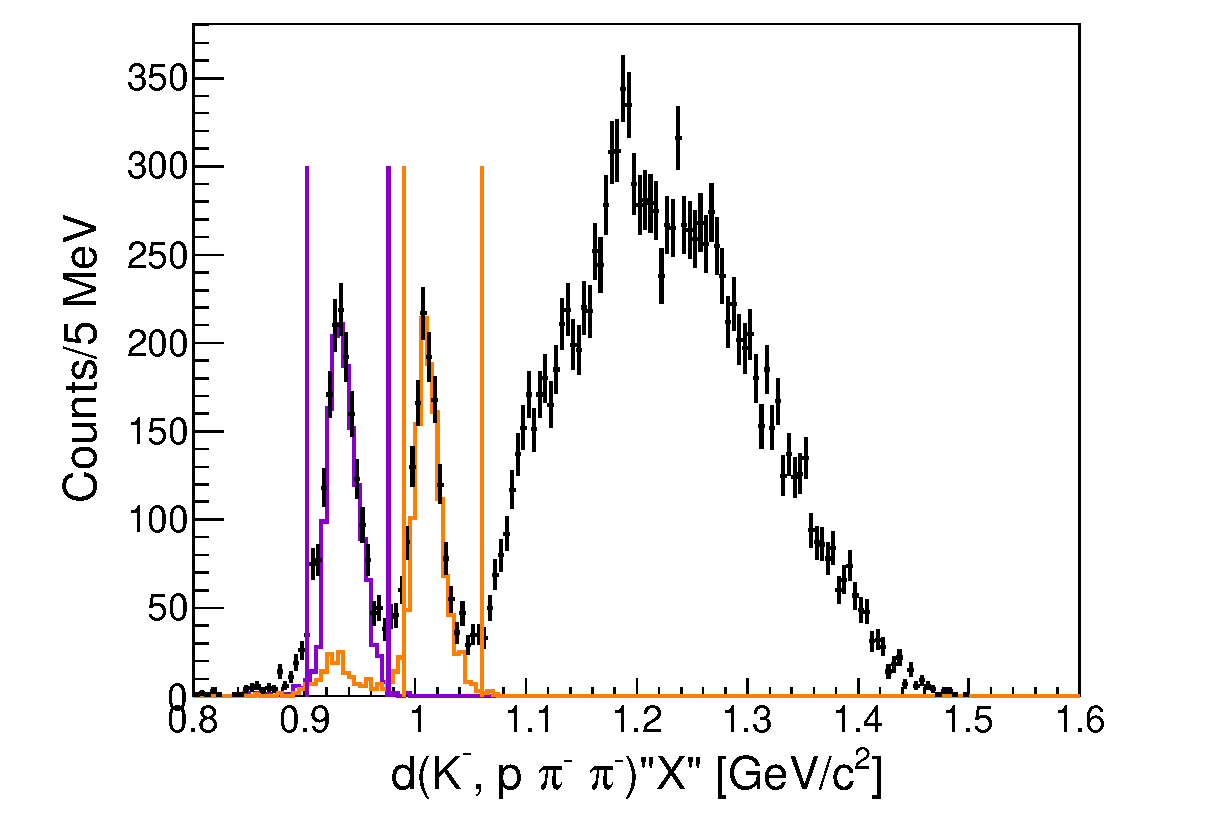
\includegraphics[width=8cm]{../pic/Run68/KP_ana/KPpimpim_MM.eps}
  \caption{
    This figure shows the missing mass of $d(K^-, p \pi^- \pi^-)$.
    Orange and purple lines indicate selection region as missing $p$ and $p \pi^-$, respectively.
    $d(K^-, p \pi^-)"\Sigma^0"$ and $d(K^-, p \pi^-)"\Lambda"$ tagged events are drawn orange and purple plot in same figure.
  }
  \label{fig:KPpimpim}
\end{figure}

\begin{figure}[htbp]
  \centering
  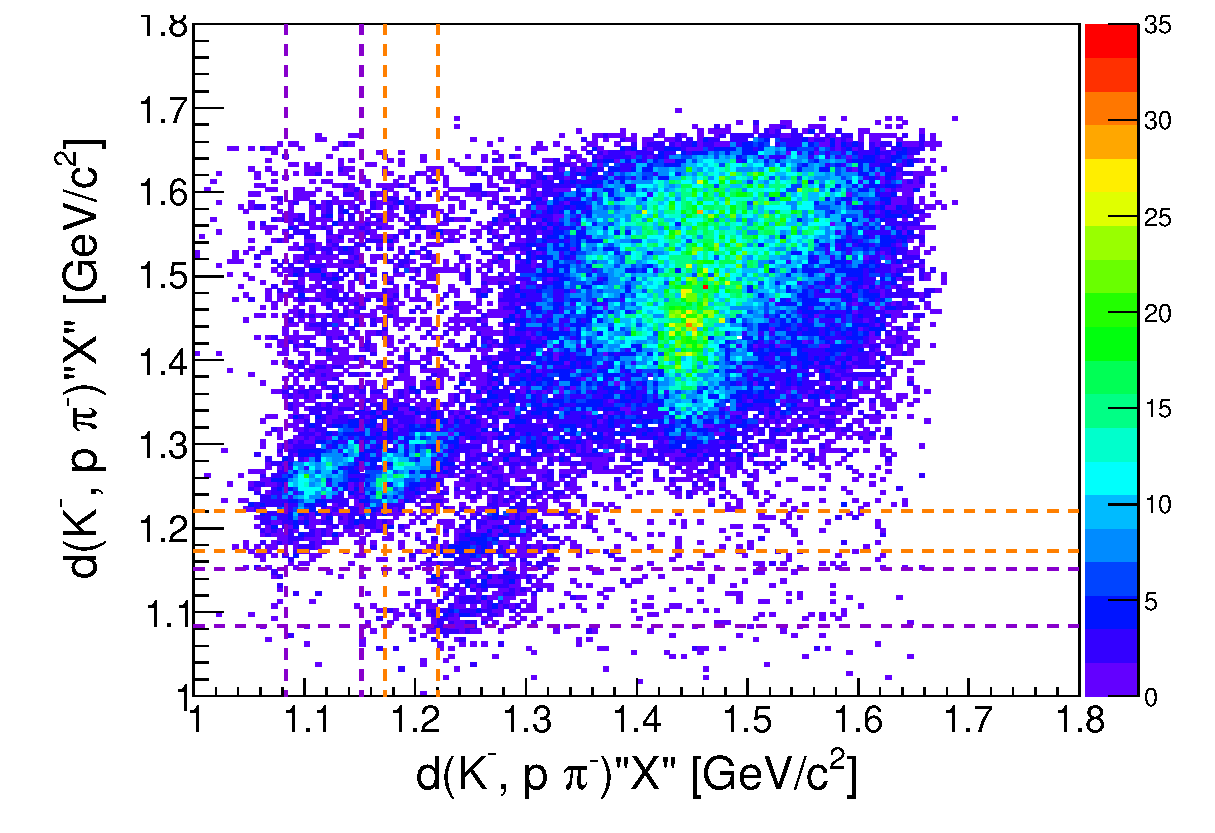
\includegraphics[width=8cm]{../pic/Run68/KP_ana/KPpim_KPpim_MM.eps}
  \caption{
    This figure shows the scatter plot of the $d(K^-, p \pi^-)$ missing masses in the $p$ and two $\pi^-$ detected events.
    Horizontal axis represents nearer DCA $\pi^-$ and virtical axis represents other one.
    Orange and purple lines indicate selection region as $d(K^-, p \pi^-)"\Sigma^0"$ and $d(K^-, p \pi^-)"\Lambda"$, respectively.
  }
  \label{fig:KPpim_KPpim}
\end{figure}


In the case of forward protons, the $\pi^-\Sigma^0$ mode is identified from the event where two $\pi^-$ are detected by the CDS.
The $\pi^-\Sigma^0$ mode has the following decay chain.
\begin{equation*}
  K^- d \rightarrow p \pi^- \Sigma^0 \rightarrow p \pi^- \Lambda \gamma \rightarrow p \pi^- \gamma p \pi^-
\end{equation*}
And $\pi^- \Lambda$ mode has a similar decay chain.
\begin{equation*}
  K^- d \rightarrow p \pi^- \Lambda \rightarrow p \pi^- p \pi^-
\end{equation*}
We identify the $\pi^-\Sigma^0$ mode by identifying $\Sigma^0$ with $d(K^-, p \pi^-)$ missing mass and $p\gamma$ with $d(K^-, p \pi^- \pi^-)$ missing mass.

The $d(K^-, p \pi^- \pi^-)$ missing mass is plotted in the Figure.\ref{fig:KPpimpim_MM},
with the $\Sigma^0$ identified from the $d(K^-, n \pi^- )$ missing mass as the orange histogram and the $\Lambda$ identified as the purple histogram.
In this reaction, $p\gamma$ make a peak like structure as this figure, because $\pi^-\Sigma^0$ momentum is small and $\gamma$ momentum is restricted.
Therefore, not only the $\pi^-\Lambda$Λ mode missin $p$ but also the $\pi^-\Sigma^0$ missing $p\gamma$ can be identified,
the range for each identification is represented by the purple and orange vertical lines.


\subsection{Mode decomposition of $d(K^-, n)$}
\begin{frame}{$d(K^-, n \pi^+ \pi^-)"X"$ data and MC (NC $\sigma=150ps$)}
  \begin{itemize}
  \item $K^- d\rightarrow (\pi^{\pm}\Sigma^{\mp})_{backwoard} n_{forward}$ (Signal)
  \item $K^- d\rightarrow K^{0} n n$ (Quasi-elastic)
  \item $K^- d\rightarrow n \pi^{\pm} \Sigma^{\mp}_{forward}$ 

  \end{itemize}
  \begin{tabular}{cc}
    \begin{minipage}{0.6\hsize}
      \begin{figure}
        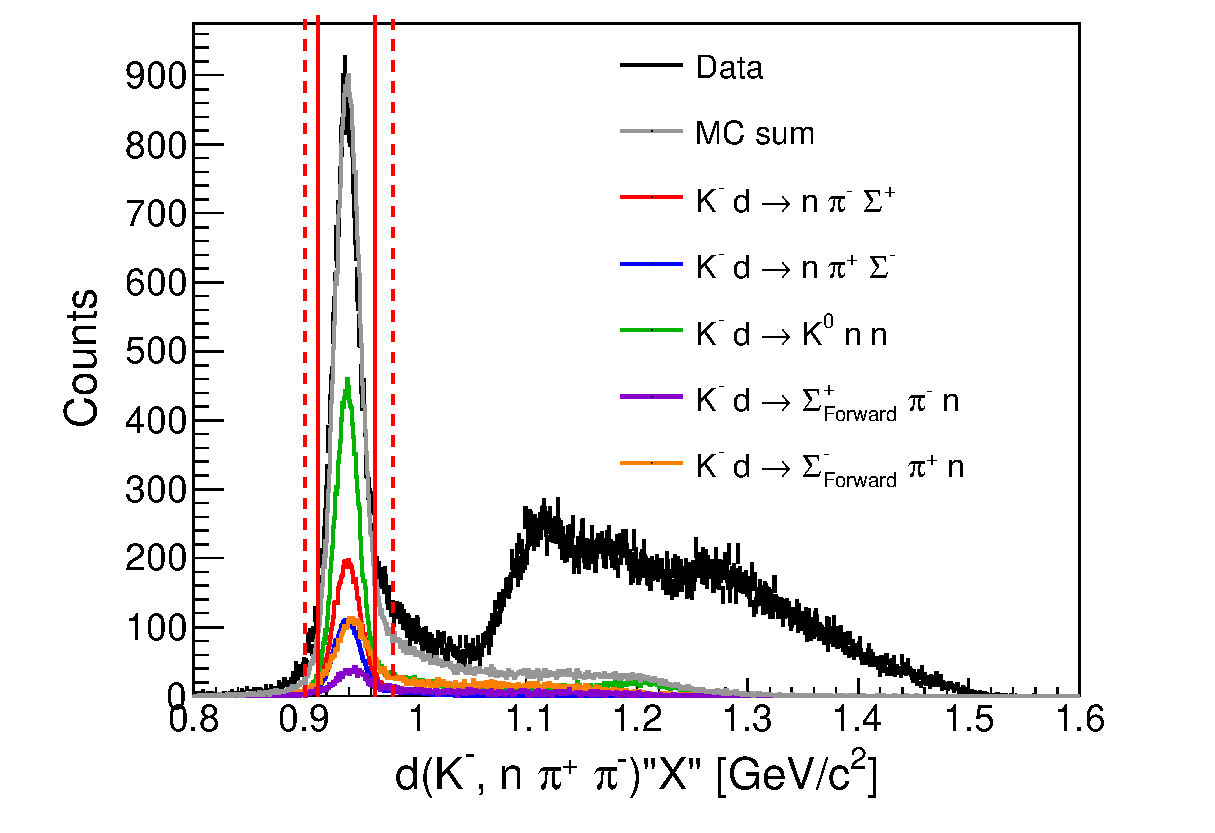
\includegraphics[width=6cm]{../pic/Run78/KN_ana_3sigma/fitKNpipi_MM.eps}
      \end{figure}
    \end{minipage}
    \begin{minipage}{0.4\hsize}
      \begin{figure}
        Data fitting\\
        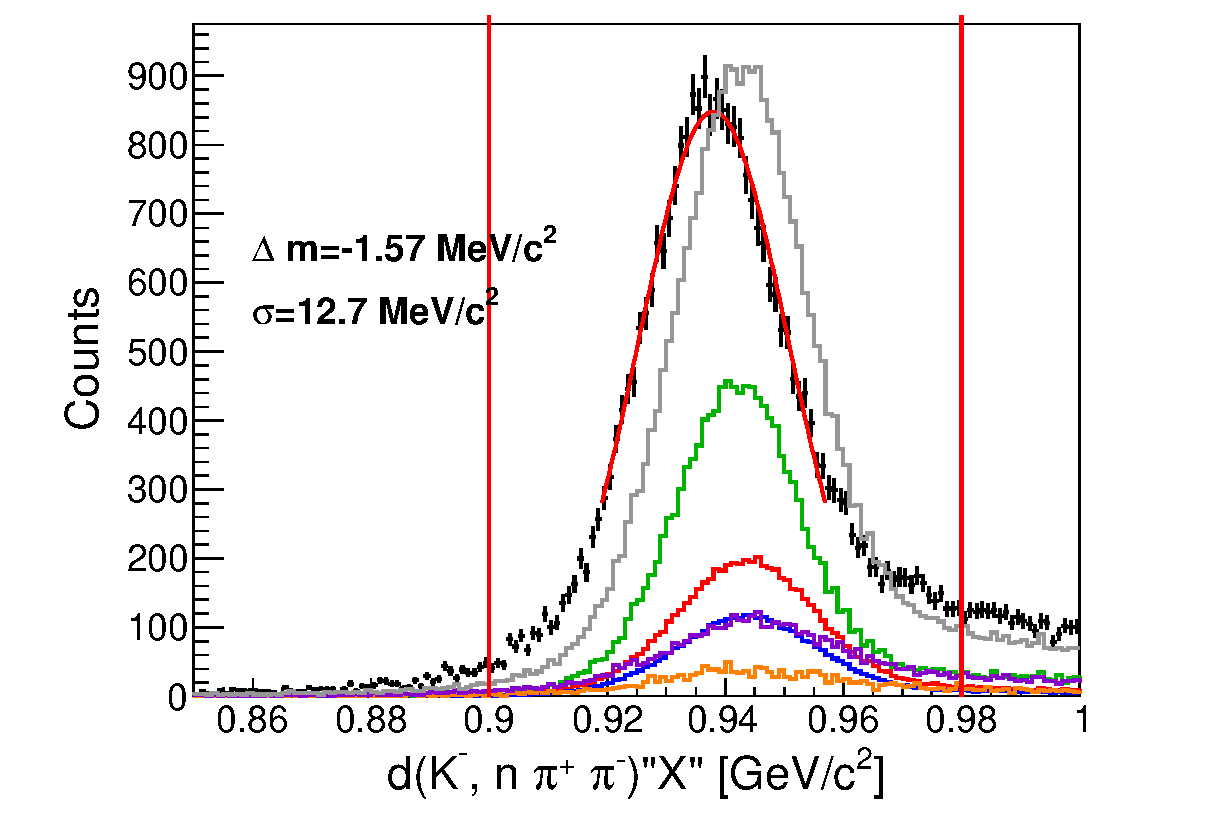
\includegraphics[width=3cm]{../pic/Run78/KN_ana_3sigma/fitKNpipi_MM_fitData.eps}\\
        MC fitting\\
        \includegraphics[width=3cm]{../pic/Run78/KN_ana_3sigma/fitKNpipi_MM_fitMC.eps}
      \end{figure}
    \end{minipage}
  \end{tabular}
\end{frame}

In the case of forward neutrons, the missing neutron is identified from the $d(K^-, n \pi^- \pi^+)$ missing mass as shown in the Figure.\ref{fig:KNpipi_MM},
and the $K^-d \rightarrow n \pi^- \pi^+ "n"$ final state is identified.
The following reactions are possible for this final state.

\begin{eqnarray}
  && K^- d \rightarrow K^0 n n \label{eq:KD_K0nn}\\
  && K^- d \rightarrow \Sigma^+_{froward} \pi^- n \label{eq:KD_pimSpf} \\
  && K^- d \rightarrow \Sigma^-_{froward} \pi^+ n \label{eq:KD_pipSmf} \\
  && K^- d \rightarrow \Sigma^+ \pi^- n_{forward} \label{eq:KD_pimSp} \\
  && K^- d \rightarrow \Sigma^- \pi^+ n_{forward} \label{eq:KD_pipSm}
\end{eqnarray}

In the reaction.(\ref{eq:KD_K0nn}) of these reactions, $K^0$ is produced and K0 decays to $\pi^+$ and $\pi^+$.
And the reacion.(\ref{eq:KD_pimSmf}) and reaction.(\ref{eq:KD_pipSpf}) produce forward charged $\Sigma$.
The neutrons measured by the forward detector are decays from the produced $\Sigma$.

These three reactions can be identified by reconstructing $K^0$ from the invariant mass of $\pi^+$ and $\pi^-$,
$\Sigma^+$ from neutron and $\pi^+$+, and
$\Sigma^-$ from neutron and $\pi^-$, as shown in the Figure.\ref{fig:KNpipi_IM}.

The remaining reactions.(\ref{eq:KD_pimSp}) and (\ref{eq:KD_pipSm}) are 2-step reactions in which the $\bar{K}$ meson kicks the neutron forward and reacts with the residual nucleon,
scattering $\pi\Sigma$ backward, which is the signal we want to measure.

\begin{figure}[htbp]
  \begin{tabular}{ccc}
    \begin{minipage}{0.33\hsize}
      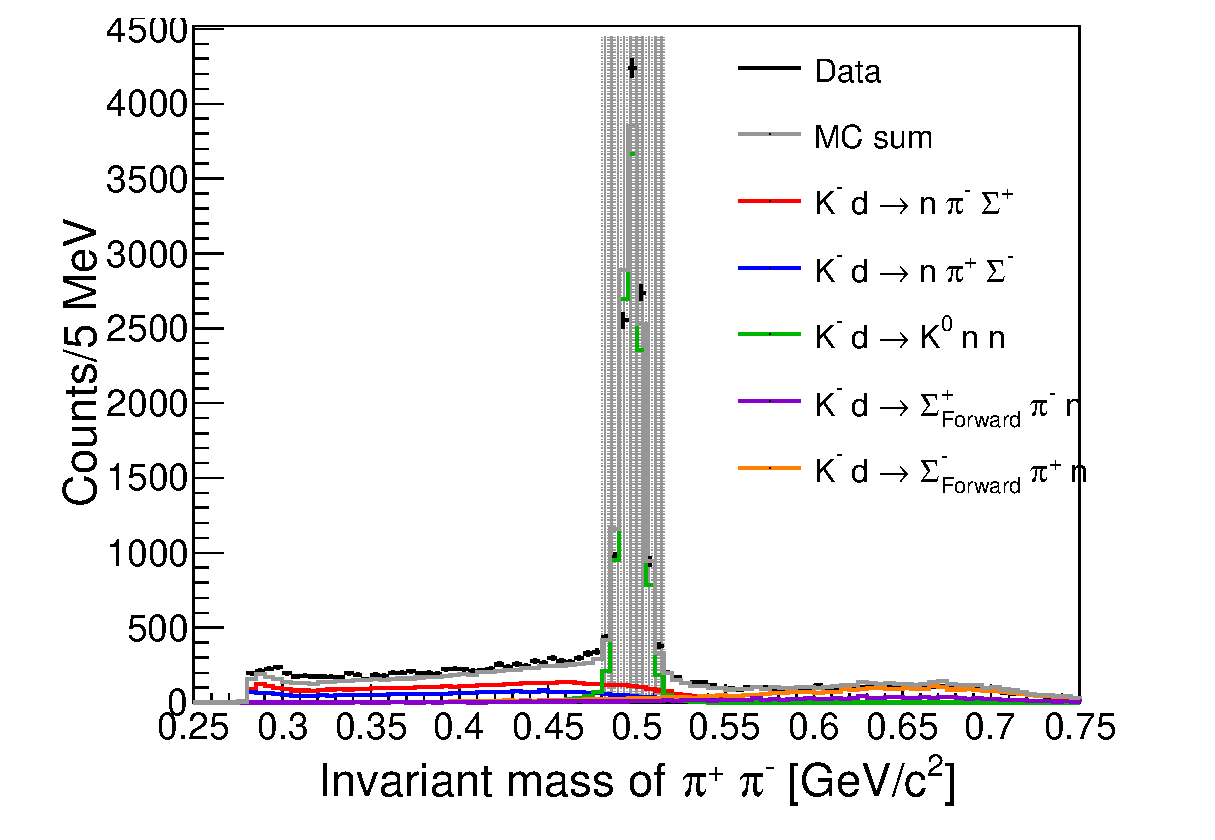
\includegraphics[width=4cm]{../pic/Run78/KN_ana_NC170_2sigma/IM_pipi.eps}
    \end{minipage}
    \begin{minipage}{0.33\hsize}
      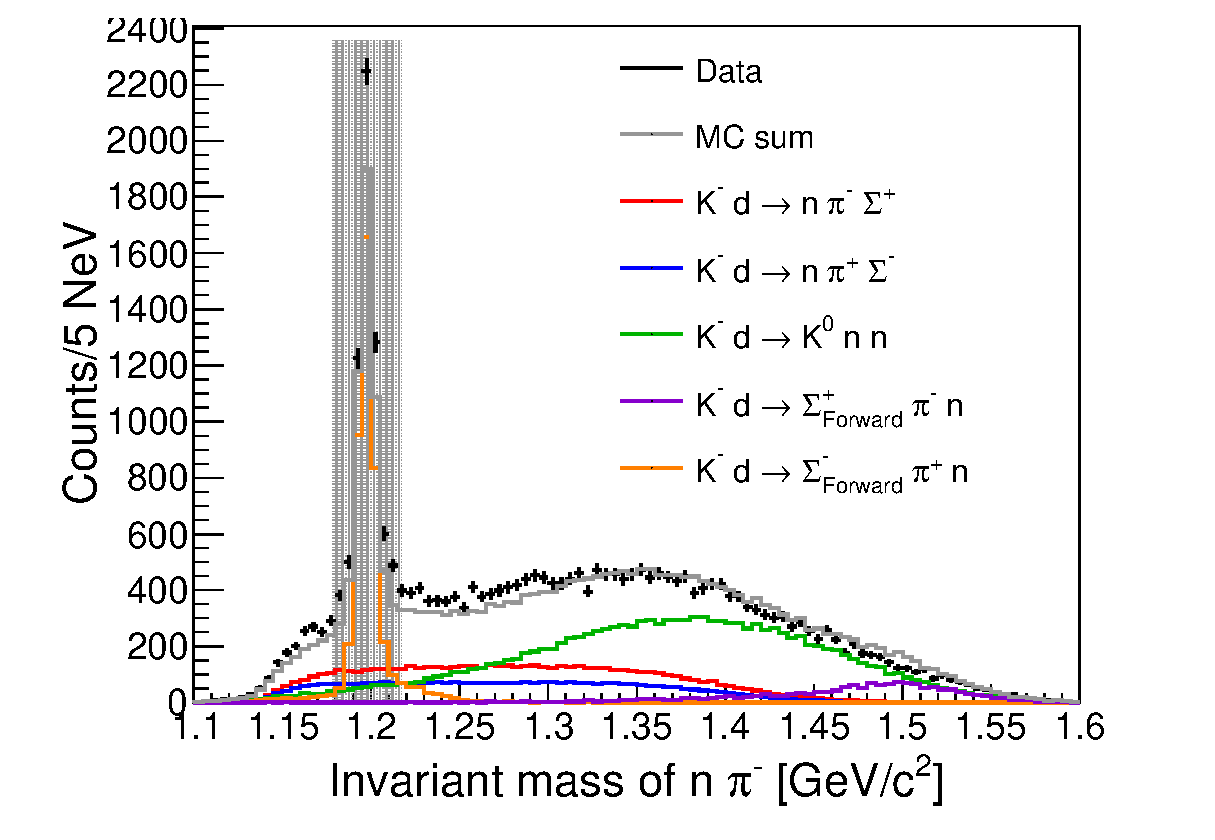
\includegraphics[width=4cm]{../pic/Run78/KN_ana_NC170_2sigma/IM_npim.eps}
    \end{minipage}
    \begin{minipage}{0.33\hsize}
      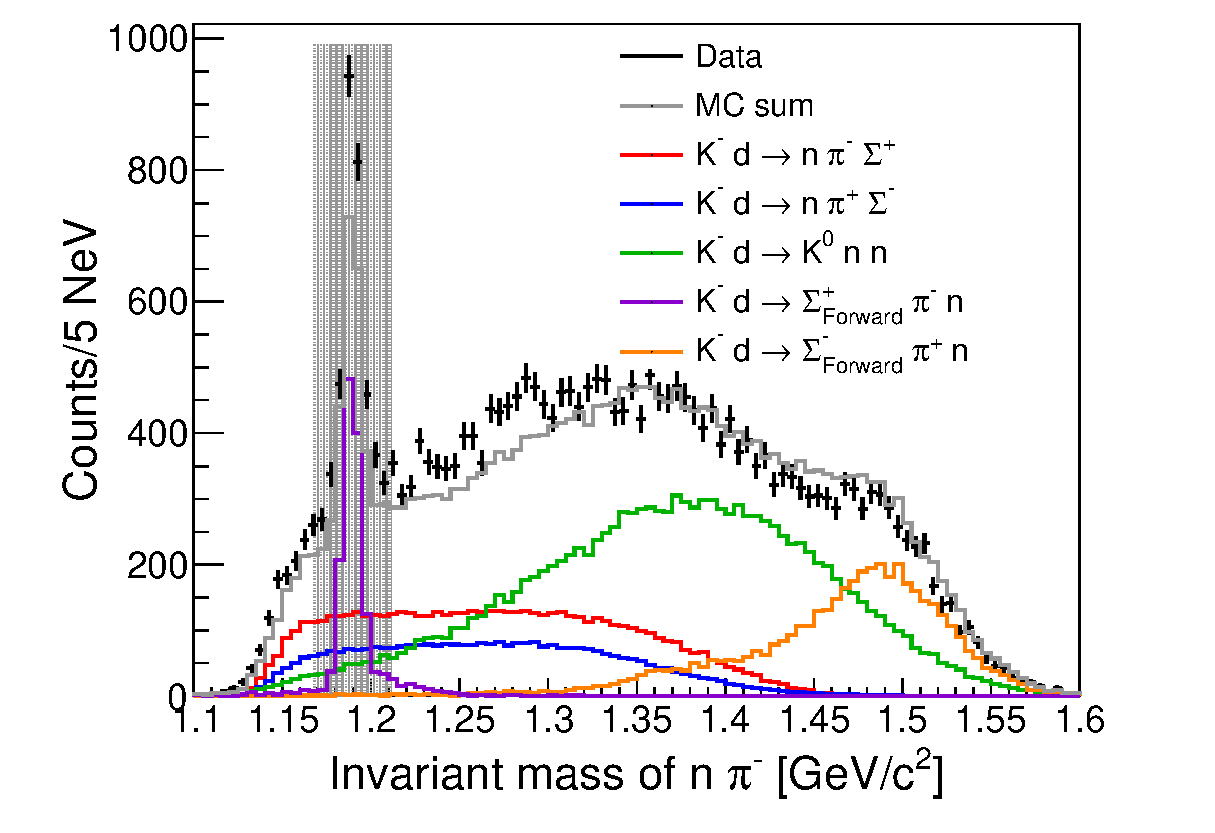
\includegraphics[width=4cm]{../pic/Run78/KN_ana_NC170_2sigma/IM_npip.eps}
    \end{minipage}
  \end{tabular}
  \caption{
    These figures shows invariant masses of $\pi^+ \pi^-$, $n \pi^-$ and $n \pi^+$ with fitting result of 5 reactions.
  }
  \label{fig:IM_fit}
\end{figure}

\begin{figure}[htbp]
\centering
  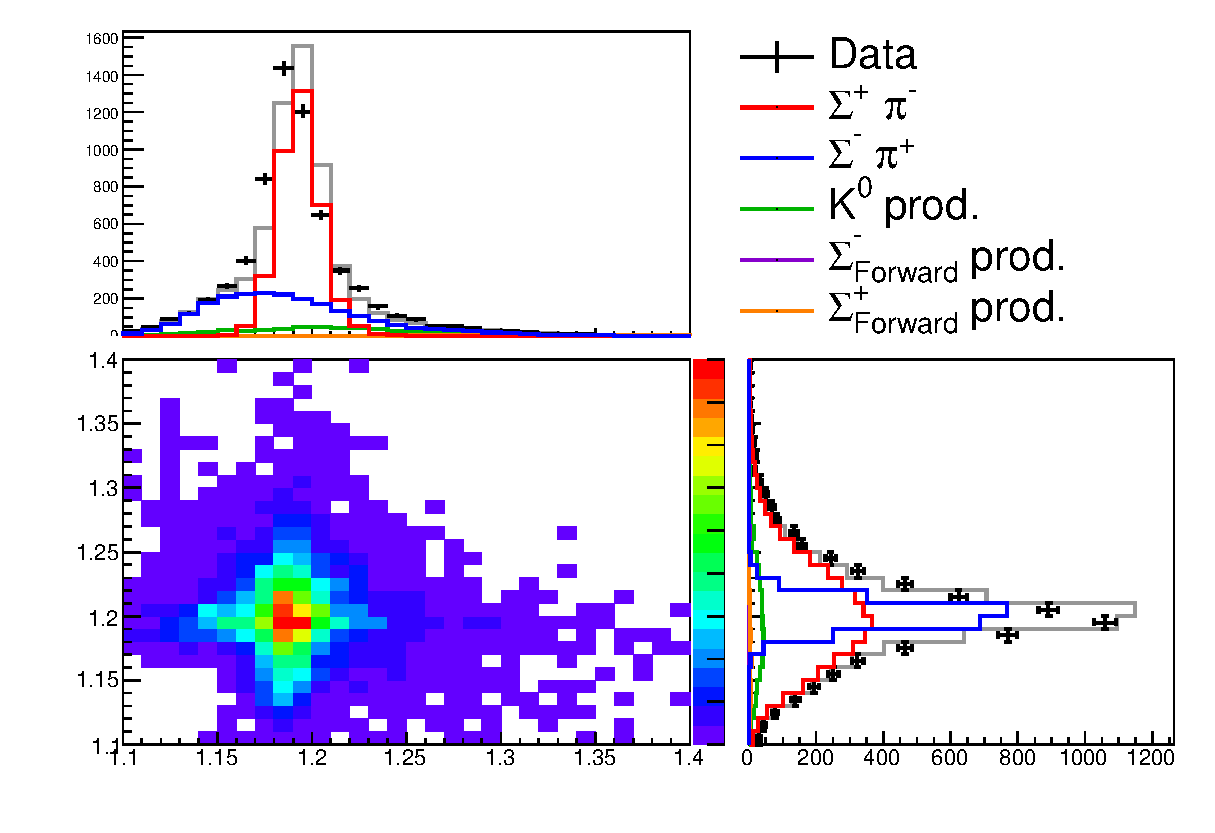
\includegraphics[width=12cm]{../pic/Run78/KN_ana_NC170_2sigma/KNpim_KNpip_MM.eps}
  \caption{
    This figure indicates summed up fitting result and log-likelihood value of each bins.
  }
  \label{fig:KNpi_MM_fit}
\end{figure}


The two modes are identified by the $d(K^-, n \pi)$ missing masses as shown in Figure.\ref{fig:KNpi_MM_all}.
In that figure for example, in the case of the $\pi^-\Sigma^+$ mode,


the missing mass of the charge opposite to $\Sigma$ results in the correct Σ peak as shown in the red line, while the missing mass of π decays from Σ and is widely distributed in the kinematically allowed region without any structure as shown in the blue line.
